\documentclass{article}
\usepackage{graphicx} % Required for inserting images
\usepackage{enumitem}
\usepackage{listings}
\usepackage{amsmath}
\usepackage{amssymb}
\usepackage[
    left=3cm,
    right=3cm,
    top=2cm,
    bottom=2cm
]{geometry}
\usepackage{titlesec}
\usepackage{microtype}

\setlength{\parindent}{0pt}
\setlength{\parskip}{6pt}
\titlespacing{\subsection}{2em}{3.25ex plus 1ex minus .2ex}{1.5ex plus .2ex}
\lstset{basicstyle=\ttfamily\small, xleftmargin=2em}

\title{
    \textbf{Introduction to Message Passing Interface} \\
    \large Graded Exercise 1
}
\author{Hai Yu}
\date{}

\begin{document}

\maketitle

\section{Introduction}

The objective of this exercise is to implement and evaluate a matrix computation
using the Message Passing Interface (MPI).

The computation involves two double-precision matrices
$\textbf{A}$ with $N=128000$ rows and $M=500$ columns,
$\textbf{B}$ with $M=500$ rows and $K=1000$ columns, and a vector
$\textbf{c}$ with $K=1000$ elements.
All elements are packed with random values between $[-1,1]$,
using predefined random seeds 10, 20 and 30.
The main task is to compute the vector
\begin{equation}
    \textbf{d = ABc},
\end{equation}
followed by its Euclidean norm,
\begin{equation}
    \mathcal{N} = \sqrt{\sum_{i=1}^{N} d_i^2}.
\end{equation}

The computation is parallelized using MPI to distribute
the workload across multiple processes with the functions
we have leant so far
\verb|MPI_*Send/MPI_*Recv|, \verb|MPI_*Bcast|, \verb|MPI_*Reduce|,
and \verb|MPI_*Allreduce|.

Performance is evaluated on the AION HPC cluster
using 1, 2, 4, 8, 16, 32, 64 and 128 MPI processes
on the reservation (\verb|mpi_course|).

Execution times are measured separately for initialization,
matrix operations and reduction operations.
The resulting measurements are used to analyze
speedup and efficiency.

\section{Explanation of the Parallelization}

The computation is performed in two stages using row-wise
matrix decomposition. Both matrices $\textbf{A}$ and $\textbf{B}$ are divided
into $P$ MPI processes, with any remaining rows assigned
to rank 0. This distributes the computational workload
while avoiding the storage of the full matrices on
worker processes.

\begin{figure}[htbp]
    \centering
    \includegraphics[
        width=\textwidth
    ]{mpi_flow.pdf}
    \caption{MPI parallel computation workflow
        for the matrix-vector operations.}
    \label{fig:mpi_workflow}
\end{figure}

\textbf{Stage 1: Computing $\textbf{x} = \textbf{Bc}$.}
Rank 0 initializes the matrices and vector, broadcasts
$\textbf{c}$ using \verb|MPI_Bcast|, and distributes blocks
of rows of $\textbf{B}$ using \verb|MPI_Send| and
\verb|MPI_Recv|. Each process computes its local
matrix-vector product by function \verb|dgemv|.

The partial results occupy disjoint positions in the
intermediate vector. An \texttt{MPI\_Allreduce} with
\texttt{MPI\_SUM} combines them and makes the complete
vector $x$ available to all processes.

\textbf{Stage 2: Computing $\textbf{d} = \textbf{Ax}$.}
The rows of $\textbf{A}$ are distributed using the same strategy.
Each process computes its local output.

It then calculates the local sum of squares using \texttt{ddot}.
Finally, \texttt{MPI\_Reduce} sums these values on
rank 0, which computes the Euclidean norm.

Execution times for initialization, matrix operations,
and reductions are measured using \texttt{MPI\_Wtime}.

\section{Explanation of the Scaling Results}

This is a strong scaling. The results are shown in Figure 2.
The initialization phase exhibits no speedup,
remaining between 0.73 and 0.84 for multiple processes,
because rank 0 initializes and distributes the matrices.

\begin{table}[htbp]
    \centering
    \label{tab:mpi_timings}
    \small
    \setlength{\tabcolsep}{5pt}
    \renewcommand{\arraystretch}{1.1}
    \begin{tabular}{r|rrrr}
        \hline
        Ranks & Initialization & Operations & Reduction & Total    \\
        \hline
        1     & 0.281032       & 0.061716   & 0.000078  & 0.342826 \\
        2     & 0.339594       & 0.030922   & 0.000137  & 0.370694 \\
        4     & 0.346939       & 0.015329   & 0.016168  & 0.389399 \\
        8     & 0.342441       & 0.007655   & 0.024105  & 0.386760 \\
        16    & 0.336465       & 0.003952   & 0.030285  & 0.386299 \\
        32    & 0.337626       & 0.001954   & 0.006728  & 0.395449 \\
        64    & 0.341865       & 0.000941   & 0.005280  & 0.406348 \\
        128   & 0.385170       & 0.000502   & 0.004575  & 0.464358 \\
        \hline
    \end{tabular}
    \caption{Execution times for different numbers of MPI processes (seconds).}
\end{table}

In contrast, the matrix operations achieve nearly linear speedup,
reaching 122.94 with 128 MPI processes. This demonstrates effective workload distribution
and good computational scalability.

\begin{figure}[htbp]
    \centering
    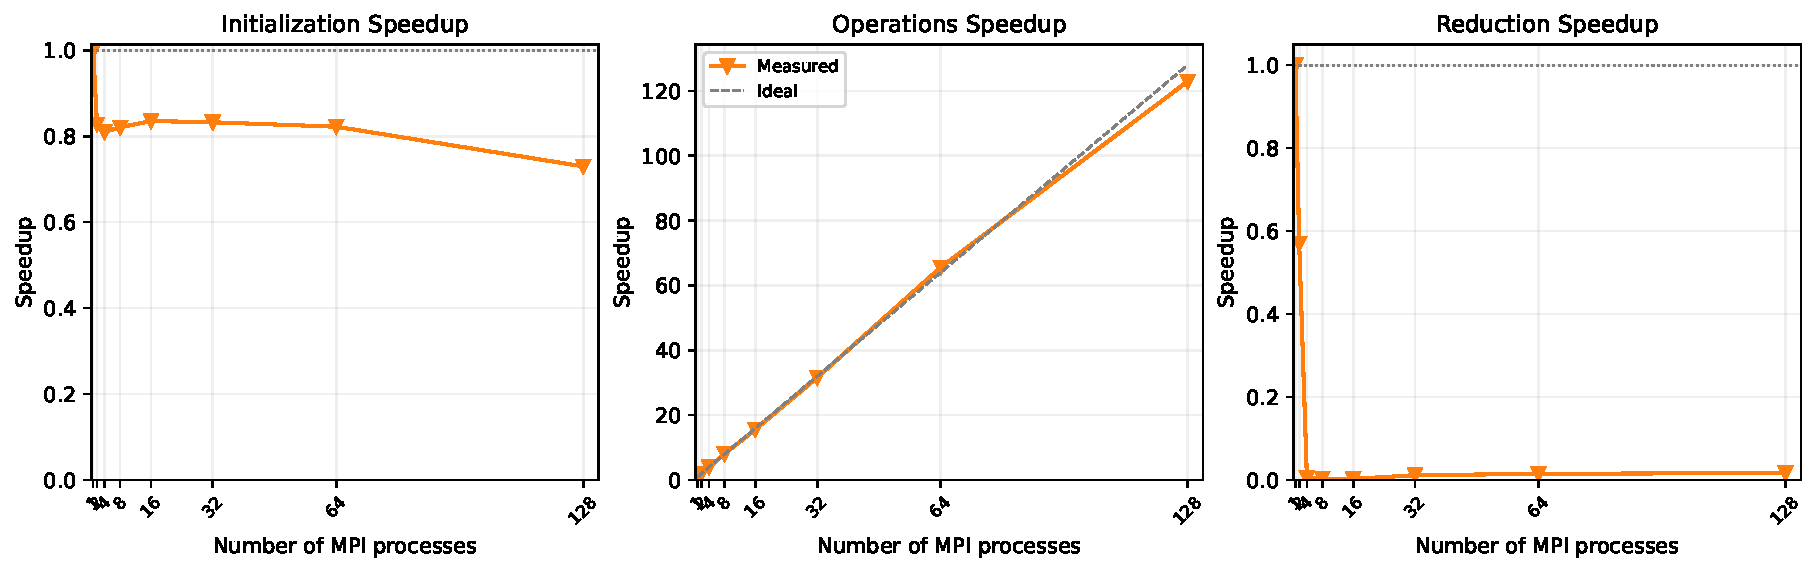
\includegraphics[width=\linewidth]
    {mpi_phase_speedup.pdf}
    \caption{Speedup of initialization, matrix
        operations, and reduction using MPI.}
    \label{fig:phase_speedup}
\end{figure}

The reduction phase shows poor scaling.
Since the single-process reduction time is extremely small,
communication and synchronization overhead dominate as
the number of processes increases. Overall, the results demonstrate
that the computational workload scales efficiently, while initialization
and collective communication limit the performance of the other phases.

\end{document}